\documentclass[tikz,border=12pt]{standalone}
\usepackage[T1]{fontenc}
\usepackage{lmodern}
\usetikzlibrary{arrows.meta,calc,positioning,shapes.geometric}

\definecolor{llmblue}{HTML}{1565C0}
\definecolor{replorange}{HTML}{E65100}
\definecolor{finalgreen}{HTML}{2E7D32}
\definecolor{warnred}{HTML}{C62828}
\definecolor{textgray}{HTML}{455A64}
\definecolor{softgray}{HTML}{ECEFF1}

\begin{document}
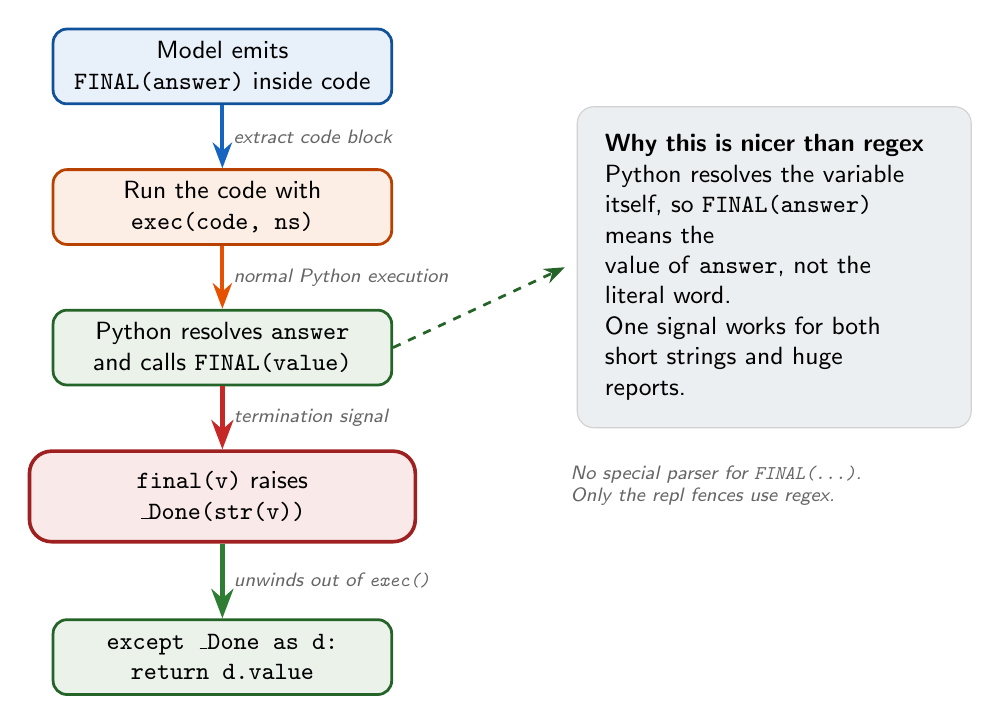
\begin{tikzpicture}[
		>=Stealth,
		font=\sffamily\small,
		block/.style={draw=#1!80!black, fill=#1!10, rounded corners=5pt,
				minimum width=4.3cm, minimum height=0.95cm, align=center,
				line width=1pt},
		note/.style={font=\sffamily\scriptsize\itshape, text=black!60, align=center},
		label/.style={font=\sffamily\scriptsize\bfseries, text=textgray},
		sidebox/.style={draw=black!18, fill=softgray, rounded corners=6pt,
				inner sep=10pt, align=left, text width=4.3cm},
	]

	\node[block=llmblue] (model) at (0, 2.9)
	{Model emits\\\texttt{FINAL(answer)} inside code};

	\node[block=replorange, below=0.8cm of model] (exec)
	{Run the code with\\\texttt{exec(code, ns)}};

	\node[block=finalgreen, below=0.8cm of exec] (call)
	{Python resolves \texttt{answer}\\and calls \texttt{FINAL(value)}};

	\node[draw=warnred!80!black, fill=warnred!10, rounded corners=8pt,
		minimum width=4.9cm, minimum height=1.15cm, line width=1.3pt,
		align=center, below=0.8cm of call] (done)
	{\texttt{final(v)} raises\\\texttt{\_Done(str(v))}};

	\node[block=finalgreen, below=0.95cm of done] (catch)
	{\texttt{except \_Done as d:}\\\texttt{return d.value}};

	\draw[->, line width=1.4pt, llmblue] (model) -- (exec)
	node[midway, right, note] {extract code block};
	\draw[->, line width=1.4pt, replorange] (exec) -- (call)
	node[midway, right, note] {normal Python execution};
	\draw[->, line width=1.7pt, warnred] (call) -- (done)
	node[midway, right, note] {termination signal};
	\draw[->, line width=1.7pt, finalgreen] (done) -- (catch)
	node[midway, right, note] {unwinds out of \texttt{exec()}};

	\node[sidebox, anchor=west] (why) at (4.5, 0.35) {
		\parbox{4.1cm}{\raggedright
			\textbf{Why this is nicer than regex}\\
			Python resolves the variable itself, so \texttt{FINAL(answer)} means the\\
			value of \texttt{answer}, not the literal word.\\
			One signal works for both short strings and huge reports.}
	};

	\draw[->, dashed, line width=1pt, finalgreen!80!black]
	(call.east) -- ([xshift=-0.15cm]why.west);

	\node[note, align=left, anchor=north west] at ([xshift=-0.2cm,yshift=-0.35cm]why.south west)
	{No special parser for \texttt{FINAL(...)}.\\Only the repl fences use regex.};

\end{tikzpicture}
\end{document}
